\chapter{5. Discussion}

\subsection{How to tackle ``relative'' valuing}
One finding is the reports are ``relative'' to the previous
experience. This is another character of the ``wicked problem'', which
``wicked problems'' are unique.\cite{rittel2973dilemmas} 
It is unique since each user may have different perceptions on bike
lane security, but more importantly, it relative to the previous set
environment.

Multiple people have commented the relativity of their perception. Data
shows that they feel insecure when bike lanes disappear.
\footnote{the intersection of Beacon Street and Bay State Street, which the
separated bike lane disappears. This separated bike lane was installed as a
response of a bike accident.}
Which we do not know whether the overall bike lane safety has improved.

The users' feedback also cast new questions on how to annotate the
city. Bikebump used a 15m radius geofence as a method, but users implied
that ``good'' situations are likely to be a continuous experience rather than
a moment reaction. Measuring methods looking at a constant input may also
validate this perception.

\section{Bottom Up design, do we care?}

It is likely that bikers are aware that the city is still dangerous and
needs improvements. Yet, none of the subjects not knowing the 
how to change the city is questioning.

One reason may be that the mental threshold of changing their city is so
costly enough that they do not even bother to know how to change.

This might be supported by the fact that younger people tend to moving more
frequently,% TODO: bib this
which whether you devote for any participatory design, you will
be living somewhere else by the time you appreciate the physical change.

\footnote{It is apparent that younger people move than the elder
  generations.
    \url{https://fivethirtyeight.com/datalab/how-many-times-the-average-person-moves/},
    yet there are reports that the rate of younger people moving is
    decreasing overtime.
    \url{http://www.nytimes.com/2012/03/11/opinion/sunday/the-go-nowhere-generation.html?_r=1&src=me&
}

This may imply that for younger generations a shorter span reward is 
preferable. We can see this by the loop of dopamine coming from the instant
gratification of peer approval in Social Media Networks. % TODO: back up

While this thesis stands on fact that the app or website is already recognized by the
user, it is important to consider how to design the initial contact.

\subsection{Initial Contact with citizens}

\textbf{Where} \\ 
In the after bike discussion, more than half of the people said that
they prefer not to have the city supervising or the planning side
set a concentration area for getting input.
People demanded a open platform that they report, propose and vote when and
where ever they wanted. On the other hand, people also recognized that if
that is the case, the likely hood of encountering to this app will be
totally by chance. This gives a possibility of how we recruit the
participants. It is easier to start from a trial that has a target path, meeting the
need from the city, and to gradually expand to a greater
audience.
This is possible, because of the mobile characteristics of the app,
and is unique compared to the traditional methods of community engagement.

\textbf{When} \\
Methods that require people to meet physically has a limit of the physical
space but time is also a constrain. It is hard to coordinate these two and
have the majority of the people building consensus.
The app can be installed and used anytime, yet the capacity of human cognition
in a given time is also limited. A survey shows that most of the Android Apps looses 77\% of the
Daily Active Users after three days.
\footnote{http://andrewchen.co/new-data-shows-why-losing-80-of-your-mobile-users-is-normal-and-that-the-best-apps-do-much-better/?utm_content=buffere4fa2&utm_medium=twitter.com&utm_source=social&utm_campaign=buffer}
It is also true that even the most dreadful natural disasters, we easily loose attraction after a short period of time.

\begin{figure}[!htb]
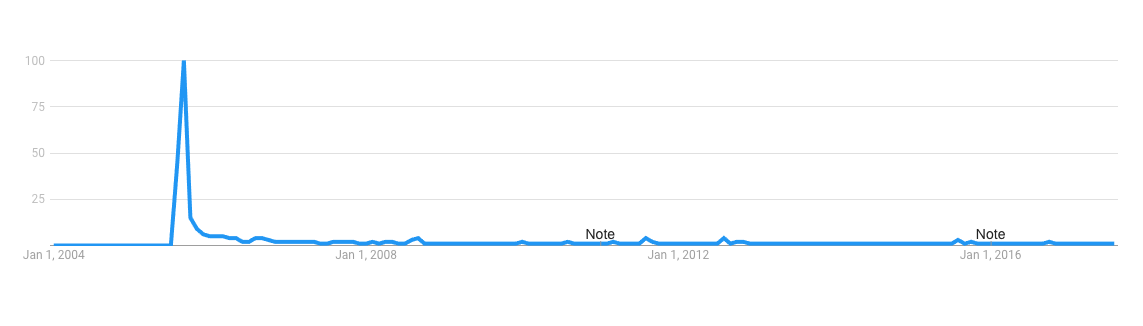
\includegraphics[width=0.6\textwidth]{chapters/5/fig/katrina_trend.png}
\caption[Trend for hurricane Katrina]{\textbf{Google Trend} number of searches for the term `Hurricane
Katrina'}
\label{fig:katrina_trend}
\end{figure}

The proposed process to incorporate Bikebump in the current TIP method still
has an annual cycle to update the list of demanding improvement proposals. Rather than releasing the app and
wait for the community to spontaneously participate, a periodic campaign
may be effective. If we think of the attention from the public as something
we need to raise, report from the Nonprofit Research Collaborative 
/footnote{/url{https://npresearch.org/pdf/2014-reports/NRC_AnnualFund_SpecialReport_July_2014.pdf}}
also points that Non Profit Organizations tend to meet their fund raising
goals from annual funds.


\subsection{Communal value to Civic value}
Shirkey points out that internet has lowered
the threshold barrier to coordinating with each other, and within this
collective action, there are two kinds of value mechanisms; Communal and
Civic values.\cite{shirky2010cognitive}

Communal value is created by and acknowledged
the same group. Although bikebump target modification in infrastructure, is
fundamentally for bikers by bikers, which makes bikebump's engine the communal value
behavior. Allowing others using different modes of transportation is the
next step for inclusion.

\subsection{Personalization}
One comment from the usertest was the personilzation of the app. The app
did not show identity.\footnote{except distinguishing individual proposals.
One concern that users will be able to identify other users homes.} Waze
uses icons to show other users in the map, aiming for the sense of
community within the people who drive in the same area.

\section{A generalized tool for collective urban design}
This thesis has been investigating a new tool for having a bottom up urban
design method. The bikebump 


definition of data collection, different modes of micro participation
A mapping of one existing situation (often unstructured / hard to grasp) to another quantifiable form (number)
\section{Micro owning the city}
Each report as declaration of ownership = share economy
\section{Scope and different application}
pedestrian sidewalks
  street lights
  regional developments

